\documentclass[12pt, openany]{book}

% ──────────────────────────────────────────────
% Packages
% ──────────────────────────────────────────────
\usepackage[margin=1in]{geometry}
\usepackage{amsmath, amssymb, amsthm}
\usepackage{mathtools}
\usepackage{bm}
\usepackage{graphicx}
\usepackage{float}
\usepackage{tikz}
\usepackage{pgfplots}
\pgfplotsset{compat=1.18}
\usetikzlibrary{arrows.meta, decorations.markings, calc, patterns, positioning}
\usepackage{tcolorbox}
\tcbuselibrary{theorems, breakable, skins}
\usepackage{hyperref}
\usepackage{enumitem}
\usepackage{fancyhdr}
\usepackage{titlesec}
\usepackage{epigraph}
\usepackage{xcolor}
\usepackage{booktabs}

% ──────────────────────────────────────────────
% Colors
% ──────────────────────────────────────────────
\definecolor{chapblue}{RGB}{0, 70, 130}
\definecolor{accentred}{RGB}{180, 40, 40}
\definecolor{softgray}{RGB}{245, 245, 245}
\definecolor{trajgreen}{RGB}{30, 130, 60}
\definecolor{darkgold}{RGB}{160, 120, 20}
\definecolor{purplehaze}{RGB}{100, 40, 140}

% ──────────────────────────────────────────────
% Theorem environments
% ──────────────────────────────────────────────
\newtcbtheorem[number within=chapter]{principle}{Principle}{
  colback=chapblue!5, colframe=chapblue!80,
  fonttitle=\bfseries, separator sign={.~},
  breakable
}{princ}

\newtcbtheorem[number within=chapter]{keyidea}{Key Idea}{
  colback=accentred!5, colframe=accentred!70,
  fonttitle=\bfseries, separator sign={.~},
  breakable
}{idea}

\newtcbtheorem[number within=chapter]{example}{Example}{
  colback=softgray, colframe=black!40,
  fonttitle=\bfseries, separator sign={.~},
  breakable
}{ex}

\newtcbtheorem[number within=chapter]{definition}{Definition}{
  colback=darkgold!5, colframe=darkgold!80,
  fonttitle=\bfseries, separator sign={.~},
  breakable
}{def}

\newtcbtheorem[number within=chapter]{remark}{Remark}{
  colback=purplehaze!5, colframe=purplehaze!60,
  fonttitle=\bfseries, separator sign={.~},
  breakable
}{rem}

\newtcbtheorem[number within=chapter]{warning}{Warning}{
  colback=accentred!5, colframe=accentred!80,
  fonttitle=\bfseries, separator sign={.~},
  breakable
}{warn}

\theoremstyle{plain}
\newtheorem{proposition}{Proposition}[chapter]
\newtheorem{theorem}{Theorem}[chapter]
\newtheorem{lemma}[theorem]{Lemma}
\newtheorem{corollary}[theorem]{Corollary}

% ──────────────────────────────────────────────
% Chapter formatting
% ──────────────────────────────────────────────
\titleformat{\chapter}[display]
  {\normalfont\huge\bfseries\color{chapblue}}
  {\chaptertitlename\ \thechapter}{20pt}{\Huge}
\titlespacing*{\chapter}{0pt}{-20pt}{30pt}

% ──────────────────────────────────────────────
% Header/Footer
% ──────────────────────────────────────────────
\pagestyle{fancy}
\fancyhf{}
\fancyhead[LE,RO]{\thepage}
\fancyhead[RE]{\textit{Control Is Motion}}
\fancyhead[LO]{\textit{\nouppercase{\leftmark}}}
\renewcommand{\headrulewidth}{0.4pt}
\setlength{\headheight}{14.5pt}

% ──────────────────────────────────────────────
% Custom commands
% ──────────────────────────────────────────────
\newcommand{\state}{\bm{x}}
\newcommand{\control}{\bm{u}}
\newcommand{\traj}{\bm{\gamma}}
\newcommand{\manifold}{\mathcal{M}}
\newcommand{\configspace}{\mathcal{Q}}
\newcommand{\statespace}{\mathcal{X}}
\newcommand{\controlspace}{\mathcal{U}}
\newcommand{\Reals}{\mathbb{R}}
\newcommand{\dd}{\mathrm{d}}
\newcommand{\dt}{\,\dd t}
\newcommand{\norm}[1]{\left\lVert #1 \right\rVert}
\newcommand{\inner}[2]{\left\langle #1,\, #2 \right\rangle}

% ──────────────────────────────────────────────
\begin{document}

\setcounter{chapter}{7}

\chapter{Phase-Variable Control}
\label{ch:phase_variable_control}

\section{Coordination, Progress, and the Clock}

Two swings can pass through similar joint configurations at different speeds and produce different impacts. Conversely, a modest delay need not spoil a shot if the golfer still reaches a suitable contact state. Phase-variable control addresses this distinction by scheduling selected relationships according to measured progress. It does not make elapsed time or velocity physically irrelevant.

For a prescribed configuration path $q_d(s)$, write $\nu=\dot s$. Its mechanically consistent lift is
\begin{equation}
q=q_d(s),\qquad v=q_d'(s)\nu,\qquad
\dot v=q_d''(s)\nu^2+q_d'(s)\dot\nu .
\end{equation}
Changing $\nu$ changes the velocity state, inertial loads, actuator demand, and impact speed. A configuration path with freely varying speed generally lifts to a two-dimensional surface in state space, parameterized by $(s,\nu)$; specifying a speed law reduces that freedom. A full-state reference $(q_d(s),v_d(s))$ already specifies velocities. It cannot generally be traversed at arbitrary speed while preserving $\dot q=v$.

This is the connection to Chapters 2 and 6: geometry organizes possible motion, while dynamics determines which timing laws can realize it. Phase scheduling can avoid an unnecessary catch-up command when a movement slows, but its performance depends on the phase estimator, feedback, and available actuation. Time tracking with a reference governor can also adapt its schedule. Neither architecture is universally safer.

\section{A Phase Coordinate Has a Domain}

On a stated region of a smooth deterministic model $\dot x=f(x)+g(x)u$, a candidate $s=\phi(x)$ has rate
\begin{equation}
\nu=\dot s=\nabla\phi(x)^\top[f(x)+g(x)u].
\end{equation}
A useful progress condition is $\nu\geq\nu_{\min}>0$ throughout the relevant closed-loop region, with the bound checked over the admitted disturbances if robustness is claimed. This is a property of the model, policy, and region together. Requiring it along every trajectory under every physically admissible control is usually unnecessarily strong and may be impossible.

If $s$ ranges from zero to one and this bound holds while solutions remain admissible, arrival takes at most $1/\nu_{\min}$. Positivity at the nominal trajectory alone does not establish the same bound for perturbed trajectories. If $\nu$ approaches zero, the change of independent variable $dx/ds=\dot x/\nu$ becomes singular; a phase-domain calculation then loses its stated justification.

A shoulder angle may reverse, a hand-path projection may repeat, and the top of a backswing may have zero angular speed. Use a restricted downswing interval, additional state information, or explicit phase charts and transition rules. A single smooth real-valued state function cannot increase strictly around an entire periodic orbit: after one period the state, and therefore that function, returns to its original value. Rhythmic models instead use a circular phase, an unwrapped phase with additional memory, or a coordinate reset.

The phase must also be estimable from the available measurements. For a local estimate $\hat x=x+\delta x$, the first-order phase error is $\delta s\approx\nabla\phi^\top\delta x$. A poorly conditioned projection amplifies measurement error; different full states with the same marker can demand different controls. Filtering trades noise against lag, and a nominally monotone marker need not remain monotone after measurement noise. Chapter 9 develops the additional changes required for a diffusion model.

\section{Virtual Constraints Live in Configuration Space}

Consider a mechanical model on a regular coordinate chart,
\begin{equation}
M(q)\ddot q+c(q,\dot q)=B(q)u ,
\end{equation}
where $M$ is positive definite and $c$ collects the stated velocity-dependent, gravitational, and other uncontrolled generalized loads. Physical loop constraints must already be reduced consistently or retained through a constrained dynamics formulation; they cannot be silently discarded.

Choose $k$ independent configuration outputs $y=h(q)$. An example is $h(q)=q_a-h_d(\phi(q))$, prescribing selected joint relationships as functions of a configuration-based phase. Here $Dh$ must have rank $k$ on the region of interest. A velocity-dependent phase generally produces a state-dependent output with different relative degree, so the configuration-only derivation below cannot be copied unchanged.

For these outputs,
\begin{equation}
\begin{aligned}
\dot y&=Dh\,v,&\ddot y&=A(q)u+b(q,v),\\
A&=Dh\,M^{-1}B,&b&=D^2h[v,v]-Dh\,M^{-1}c .
\end{aligned}
\end{equation}
The Hessian term includes the acceleration generated by moving along a curved constraint. Omitting it incorrectly treats a curved joint relationship as a straight one. The zero-output state set is
\begin{equation}
\mathcal Z=\{(q,v):h(q)=0,\ Dh(q)v=0\}.
\end{equation}
Both position and velocity conditions are necessary. Starting with $y(0)=0$ and $\dot y(0)\ne0$ gives $y(t)=t\dot y(0)+O(t^2)$, so the state immediately leaves the configuration constraint. Under the stated regularity conditions, $\mathcal Z$ has dimension $2(n-k)$ for $n$ configuration coordinates.

The term virtual means that actuation maintains the relationship. It does not mean that software creates an exact mechanical linkage under disturbances, saturation, delay, or imperfect state estimation. A physical ideal linkage supplies constraint reactions through a different force channel. Its feasibility and power properties cannot simply be assigned to a virtual constraint.

\section{Feedback Requires Input Authority}

If the number of independent inputs equals $k$ and $A$ is nonsingular, the ideal feedback
\begin{equation}
u=A^{-1}\bigl[-b-K_d\dot y-K_p y\bigr]
\end{equation}
produces $\ddot y+K_d\dot y+K_p y=0$. Positive diagonal gains give decaying output errors in this exact, unsaturated model. The on-manifold input is $u^\star=-A^{-1}b$. Its existence within the allowed input set must be checked throughout the proposed region, including any muscle activation or force-rate dynamics represented by the effective plant.

Rank loss of $A$ prevents this inversion. Near rank loss, the required commands and sensitivity to estimation error can become large. With additional inputs, a right inverse and a null-space allocation may be available, but the allocation must satisfy bounds. With too few independent input directions, the prescribed output accelerations may be infeasible. A small tracking error is not evidence that all joint torques are independently controllable.

This connects virtual constraints to underactuation rather than eliminating it. The controlled outputs consume input authority; the remaining dynamics still determine progress, energy, and internal motion. High gains also increase sensitivity to noisy differentiated measurements and can push the controller into saturation, invalidating the exact output equation.

\section{Perfect Coordination Can Hide Unstable Motion}

Consider the dimensionless two-coordinate system
\begin{equation}
\ddot q_1=u,\qquad \ddot q_2=q_2,\qquad y=q_1-q_2 .
\end{equation}
The input $u=q_2-2\dot y-y$ gives $\ddot y+2\dot y+y=0$. Output errors decay. Nevertheless, on $\mathcal Z$ the coordinates satisfy $q_1=q_2$ and the internal dynamics remains $\ddot q_2=q_2$. With $q_2(0)=\dot q_2(0)=1$, both coordinates follow $e^t$. Coordination is exact while the state grows without bound.

The example separates three claims: invariance of $\mathcal Z$, attraction of output errors toward zero, and acceptable dynamics within $\mathcal Z$. Establishing the first two does not establish the third. In a golf model, correlated joint angles could coexist with insufficient club speed, excessive speed, loss of balance, or a wrong face orientation. The task determines which internal motions are acceptable.

Nor does a virtual constraint make the remaining motion passive. For $\ddot q_1=u$, $\ddot q_2=0$, choose $h=q_1-q_2^2$. On $\mathcal Z$,
\begin{equation}
q_1=q_2^2,\qquad v_1=2q_2v_2,\qquad u^\star=2v_2^2 .
\end{equation}
With unit masses and no potential energy, $E=(v_1^2+v_2^2)/2$ and $\dot E=v_1u^\star=4q_2v_2^3$. At $q_2=v_2=1$, the controller supplies power $4$ in the example's units while the virtual constraint is satisfied exactly. An ideal stationary physical constraint force of the form $Dh^\top\lambda$ instead has power $\lambda^\top Dh\,v=0$ on its constraint. These are different actuation mechanisms.

\begin{figure}[H]
\centering
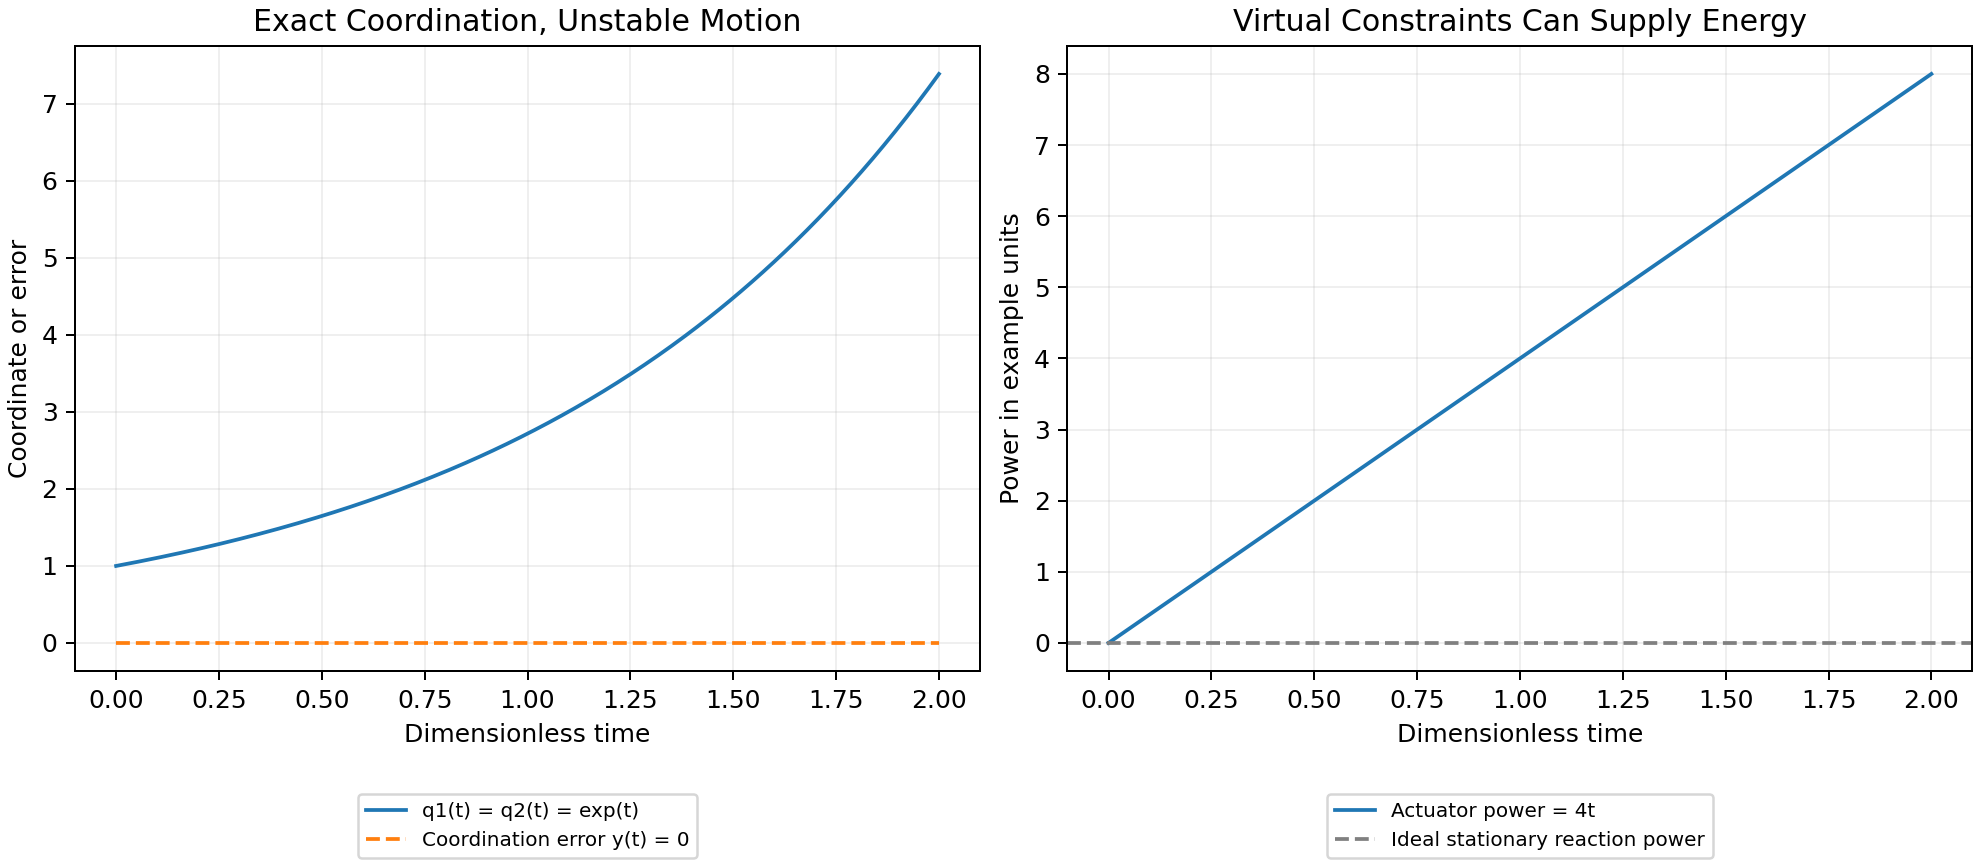
\includegraphics[width=\linewidth]{../The_Geometry_of_Motion/figures/phase_coordination_limits.png}
\caption{Coordination Does Not Determine Internal Motion}
\end{figure}

The left panel plots the exactly coordinated but unstable solution. The right panel evaluates the active power needed to maintain the parabolic virtual constraint with $q_2(0)=0$ and $v_2=1$. Both are analytic examples, not simulated human swings.

\section{Impact Adds a Separate Invariance Condition}

A hybrid model follows continuous dynamics until a guard $\mathcal S$ is reached and then applies a reset $x^+=\Delta(x^-)$. Hybrid zero dynamics requires continuous invariance and the additional condition
\begin{equation}
\Delta(\mathcal S\cap\mathcal Z^-)\subseteq\mathcal Z^+ .
\end{equation}
The pre- and post-impact output relationships can differ. The reset must preserve the appropriate position and velocity constraints, not merely make the configuration look similar.

For illustration, an instantaneous perfectly plastic contact at unchanged configuration has
\begin{equation}
\begin{aligned}
M(v^+-v^-)&=J^\top\Lambda,\qquad Jv^+=0,\\
v^+&=\left[I-M^{-1}J^\top(JM^{-1}J^\top)^{-1}J\right]v^- ,
\end{aligned}
\end{equation}
assuming independent contact rows, no other impulsive loads, and a valid sticking contact mode. This follows by solving the impulse balance and the post-impact velocity condition. A rigid ground can exchange momentum with the modeled body: its momentum is not generally conserved in isolation.

For unit mass coordinates and $J=(0,1)$, the reset changes $(v_1,v_2)=(1,1)$ to $(1,0)$. A pre-impact virtual relationship $v_1-v_2=0$ is therefore broken. Continuous output regulation did not guarantee hybrid invariance.

Club-ball contact needs its own model: normal restitution or compliant deformation, tangential interaction, spin, contact location, and any retained external impulse. The perfectly plastic sticking example is not a club-ball impact law. The first contact event must also be detected with the intended crossing direction, rather than selecting an arbitrary intersection of a plotted path.

Even valid hybrid zero dynamics does not prove stable walking. Existence of a periodic solution, admissible contacts, progress, and stability of the relevant return map require separate analysis; attraction of the transverse output dynamics must be connected to that analysis. For a single golf strike, periodic stability is usually the wrong objective. The relevant questions concern finite-time contact, ball-launch outputs, and an admissible continuation after impact.

\section{Connecting Phase Control to a Golf Outcome}

Suppose a downswing model uses $s=\phi(q)$ to schedule selected arm and club relationships. First choose the modeled interval and show that the progress coordinate remains usable there. Then check $A(q)$ and the commanded forces or torques, including passive wrist assumptions, bilateral hand closure, ground contacts, and the declared actuator dynamics. A reference satisfying a geometrical relationship but requiring unavailable torque is not a realizable swing.

Next retain the internal speed and energy variables. On a given configuration path, kinetic energy is
\begin{equation}
T(s,\nu)=\tfrac12\nu^2 q_d'(s)^\top M(q_d(s))q_d'(s).
\end{equation}
Doubling phase speed quadruples this kinetic energy at the same configuration. Clubhead velocity also scales with $\nu$ for that path. Equal phase and small output errors therefore do not imply equal impact. Impact evaluation must include clubface pose, relative contact velocity, strike location, and the chosen ball-launch or shot-loss objective.

A phase-indexed containment function $V(x,s)\leq\rho(s)$ must be differentiated with the actual phase rate:
\begin{equation}
\frac{d}{dt}\bigl[V(x,s)-\rho(s)\bigr]
=V_x\dot x+\bigl(V_s-\rho'(s)\bigr)\nu .
\end{equation}
Replacing $\nu$ by one without changing the dynamics is a different model. A tube can contain errors while the swing stalls; a progress condition is needed for arrival. A tube can reach contact while admitting poor face orientation; terminal output bounds are needed for accuracy. These are the same separate requirements developed in Chapters 4 and 7.

The biological interpretation is a testable hypothesis: scheduling coordination by a reliably estimated progress variable may reduce sensitivity to some timing disturbances. Test it against alternatives with the same actuator limits, sensing delay, initial-state distribution, and task objective. Compare held-out impact outcomes as well as joint tracking error. Observing a common joint-angle relationship does not identify the nervous system's controller or establish that it explicitly implements a virtual constraint.

\section{Primary Reading}

\href{https://grizzle.robotics.umich.edu/files/HZD_HandbookApril2015.pdf}{Grizzle and Chevallereau's virtual-constraints chapter} develops configuration outputs, the decoupling condition, zero dynamics, and hybrid invariance for underactuated locomotion. Its walking-specific results require their stated hypotheses when applied to another mechanism. The examples and golf analysis above explicitly separate those ingredients rather than asserting that locomotion results transfer automatically.

\begin{samepage}
\section{Worked Checks and Exercises}

\begin{enumerate}[itemsep=0.25em,parsep=0pt]
\item Differentiate $q_d(s(t))$ twice. Identify the terms lost by treating a curved path as a velocity reference with arbitrary timing.
\item Prove that a smooth real-valued state function cannot increase strictly around a closed periodic orbit.
\item Show that $h=0$ alone does not define the zero dynamics for a relative-degree-two output.
\item Derive the feedback for $y=q_1-q_2$ and verify the exact unstable internal solution.
\item Calculate the input and mechanical power on $q_1=q_2^2$ when $v_2$ is constant.
\item Derive the plastic-contact reset and test whether it preserves $v_1-v_2=0$.
\item For a proposed swing phase, state the measurements, monotonicity region, reset rules, and behavior if progress stops.
\item Explain why an invariant coordination surface, a successful contact event, and a stable periodic orbit are distinct claims.
\end{enumerate}
\end{samepage}

\end{document}
